\chapter{Wireframes} \label{cha:wireframes}

\section{Hoofdframe} \label{sec:hoofdframe}
\begin{figure}[h]
  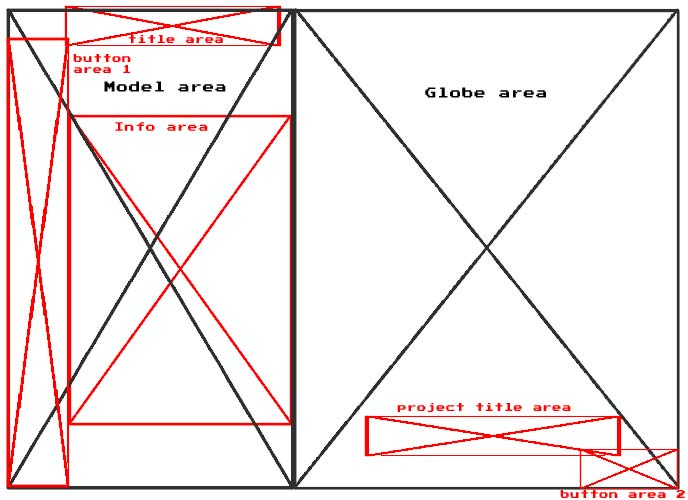
\includegraphics[width=100mm]{figs/wireframe1.jpg}
  \caption{Wireframe 1 \textit{(27-April-2014)}}
  \label{fig:wireframe1}
\end{figure}

De onderste laag is getekend in zwart, de bovenste laag is getekend in het rood.\\
De model area en globe area zijn de de belangrijkste componenten en bevatten de gehele inhoud van deze applicatie.\\
Binnen de globe area staan de project title area en de info area. De project title area is zichtbaar boven de globe area en de info area bevind zich als top laag boven alles indien zichtbaat. De project title area bevat de naam van het project, \projectname.
De inhoud van de areas zal in detail worden beschreven in \cref{cha:componenten} \nameref{cha:componenten}.
\newpage
\section{Info area wireframe} \label{sec:infowire}
\begin{figure}[h]
  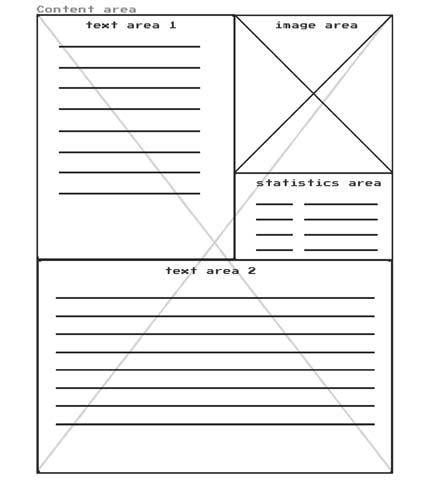
\includegraphics[width=100mm]{figs/wireframe2.jpg}
  \caption{Wireframe 2 (info area)\textit{(27-April-2014)}}
  \label{fig:wireframe2}
\end{figure}

Dit is een uitgewerkte wireframe van de info area. Dit paneel verschijnt zodra een monument wordt geselecteerd. Dit paneel kan worden gesloten met een muisklik op de knop rechtsboven in het paneel, weergegeven in het rood. In de title area staat de naam van het geselecteerde monument. In de content area komt samengevatte informatie te staan. Binnen de content area is ruimte voor text, een foto van het monument en enkele statistieken. Deze statistieken zijn gebonden aan het monument, zoals bijvoorbeeld: bouwjaar, architect en locatie gegevens. en geen ander monument kan worden gekozen terwijl het info paneel is geopend.
\newpage
